\begin{ZhChapter}

\chapter{緒論(大標)}

\section{研究動機與背景(小標)}


科技的快速進步,讓人們的生活更加便利,物聯網(IoT)的應用已經與日常生活密不可分,包含了醫療及工業的應用,無所不在,
\cite{mordor2024iot}根據日商環球訊息有限公司(GII)調查,物聯網(IoT)市場規模預計從2024年到2029年,將從1.17兆美元增加至2.37兆美元,
年均複合成長率(CAGR)為15.12\%,如(圖1.1)所示。

\begin{figure*}[htbp]
    \centering
    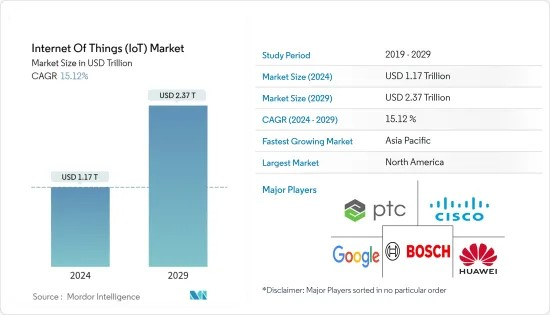
\includegraphics[width = 1\textwidth]{image/market_research.jpg}
    \caption{IoT市場規模評估\cite{mordor2024iot}}
    \label{fig: IoT市場規模評估}
\end{figure*}

2010年6月藍芽技術聯盟(Bluetooth Special Interest Group)提出了低功耗藍芽(Bluetooth Low Energy, BLE),
BLE省電及低成本的特性,使得藍芽技術在物聯網(IoT)的應用種佔據了不可或缺的角色,例如:目前市面上的無線設備包括藍芽耳機、藍芽鍵盤及藍芽滑鼠。
物聯網(IoT)的應用中,大量使用無線感測網路(Wireless Sensor Networks, WSN),會在環境之中分布許多的節點,
而節點不只有當作感知器測量環境的數據,常常還要當作中繼節點,轉傳發送端與目的端的封包,最終將所有量測的數據匯集到終端節點,
以監控所有的節點數據,將數據儲存後,進行分析後並做出適當的處理,也可以透過分析數據預測環境的變化,並提前做出適當的處理。


藍芽網狀網路(Bluetooth Mesh)架構的實現,讓BLE更具有可靠性(Reliability)及擴展性(Scalability),
可以允許多個BLE相互連接並形成網狀結構,讓封包可以在多個裝置或節點之間進行傳輸,讓傳輸距離不會受到單一裝置的傳輸範圍限制,
解決了節點之間裝置連接數量的限制以及傳輸距離不足的問題,在物聯網(IoT)的應用,
例如:智慧建築、智慧工業、智慧城市、智慧家庭..等等,BLE都已經扮演重要也不可或缺的角色。
	
在物聯網(IoT)與藍芽網狀網路(Bluetooth Mesh)中,對整個系統架構做出適當的評估,在不影響裝置效能的情況下,
設計多個藍芽裝置之間的分流機制,因為在整個系統中,流量可能會有所起伏,為了讓每個裝置可以有一樣的傳輸品質,且系統可以發揮最好的吞吐量。
	


\subsection{研究背景(小小標)}

\text 背景內文背景內文背景內文背景內文,背景內文背景內文背景內文背景內文背景內文背景內文,如表 1.1 所示。

\begin{table*}[htbp]
    \centering
    \caption{表格範例標題} \label{tab: complexity}
    \makebox[\linewidth][c]{
    \renewcommand\arraystretch{1.2}{
        \begin{tabular}{| l | c  c  c  c |}
        \hline
        Protocol & $P$ & $CS_1$ & $CS_2$ & $RG$ \\
        \hline
        SD & $O(1)$, $O(1)$, N/A & $O(n-t)$, $O(1)$, N/A & $O(n-t)$, $O(1)$, N/A & $O(1)$, $O(n)$, $O(n)$ \\
        MSSMul & $O(1)$, $O(1)$, N/A & $O(n-t)$, $O(n)$, $O(1)$ & $O(n-t)$, $O(n)$, N/A & $O(1)$, $O(n)$, $O(n)$ \\
        MSSAdd & $O(1)$, $O(1)$, N/A & $O(n-t)$, $O(n)$, $O(1)$ & N/A, N/A, N/A & $O(1)$, $O(n)$, $O(n)$ \\
        SC & $O(1)$, $O(1)$, N/A & $O(n-t)$, $O(n)$, $O(1)$ & $O(n-t)$, $O(n)$, N/A & $O(1)$, $O(n)$, $O(n)$ \\
        \hline 
        \end {tabular}
    }}
\end {table*}

\subsubsection{研究動機(小小標)}

\begin{equation} 
    \mbox{$(1+x)^n = 1 + \dfrac{nx}{1!} + \dfrac{n(n-1)x^2}{2!}$}
\end{equation}

動機動機動機動機,動機動機動機動機動機動機動機動機動機動機動機動機,動機動機動機動機動機動機動機動機。

動機動機動機動機動機動機動機動機,動機動機動機動機動機動機動機動機動機動機動機動機。動機動機動機動機動機動機動機動機,動機動機動機動機動機動機動機動機動機動機動機動機。動機動機動機動機動機動機動機動機,動機動機動機動機動機動機動機動機動機動機動機動機,如圖 1.1、圖 1.2 所示。

\begin{figure*}[htbp]
    \centering
    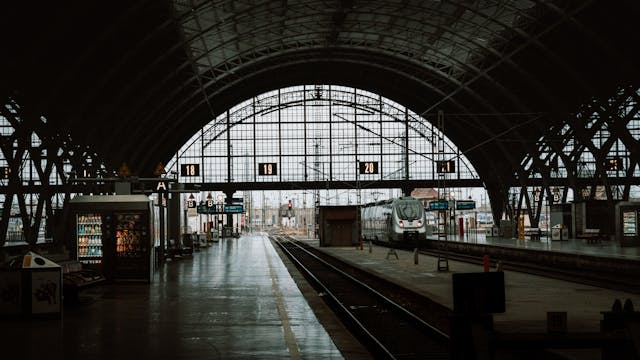
\includegraphics[width = 1\textwidth]{image/image.jpeg}
    \caption{Cool train station}
    \label{fig: image}
\end{figure*}

\begin{figure*}[htbp]
    \centering
    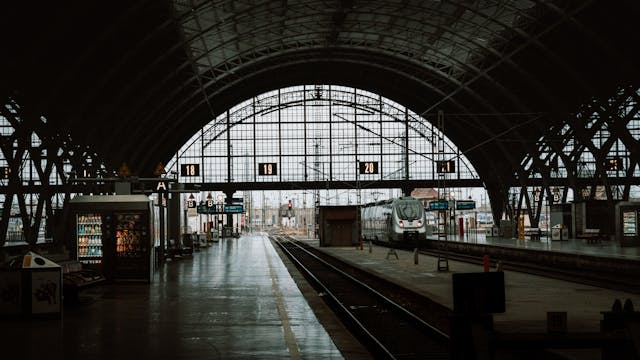
\includegraphics[width = 1\textwidth]{image/image.jpeg}
    \caption{Cool train station}
    \label{fig: image}
\end{figure*}

\begin{table*}[htbp]
    \centering
    \caption{表格範例標題} \label{tab: complexity}
    \makebox[\linewidth][c]{
    \renewcommand\arraystretch{1.2}{
        \begin{tabular}{| l | c  c  c  c |}
        \hline
        Protocol & $P$ & $CS_1$ & $CS_2$ & $RG$ \\
        \hline
        MSSMul & $O(1)$, $O(1)$, N/A & $O(n-t)$, $O(n)$, $O(1)$ & $O(n-t)$, $O(n)$, N/A & $O(1)$, $O(n)$, $O(n)$ \\
        MSSAdd & $O(1)$, $O(1)$, N/A & $O(n-t)$, $O(n)$, $O(1)$ & N/A, N/A, N/A & $O(1)$, $O(n)$, $O(n)$ \\
        SC & $O(1)$, $O(1)$, N/A & $O(n-t)$, $O(n)$, $O(1)$ & $O(n-t)$, $O(n)$, N/A & $O(1)$, $O(n)$, $O(n)$ \\
        MSSMul & $O(1)$, $O(1)$, N/A & $O(n-t)$, $O(n)$, $O(1)$ & $O(n-t)$, $O(n)$, N/A & $O(1)$, $O(n)$, $O(n)$ \\
        MSSAdd & $O(1)$, $O(1)$, N/A & $O(n-t)$, $O(n)$, $O(1)$ & N/A, N/A, N/A & $O(1)$, $O(n)$, $O(n)$ \\
        SC & $O(1)$, $O(1)$, N/A & $O(n-t)$, $O(n)$, $O(1)$ & $O(n-t)$, $O(n)$, N/A & $O(1)$, $O(n)$, $O(n)$ \\
        \hline 
        \end {tabular}
    }}
\end {table*}

動機動機動機動機,動機動機動機動機動機動機動機動機動機動機動機動機,動機動機動機動機動機動機動機動機。

動機動機動機動機,動機動機動機動機動機動機動機動機動機動機動機動機,動機動機動機動機動機動機動機動機。動機動機動機動機,動機動機動機動機動機動機動機動機動機動機動機動機,動機動機動機動機動機動機動機動機。

動機動機動機動機,動機動機動機動機動機動機動機動機動機動機動機動機,動機動機動機動機動機動機動機動機。動機動機動機動機,動機動機動機動機動機動機動機動機動機動機動機動機,動機動機動機動機動機動機動機動機。動機動機動機動機,動機動機動機動機動機動機動機動機動機動機動機動機,動機動機動機動機動機動機動機動機。

動機動機動機動機,動機動機動機動機動機動機動機動機動機動機動機動機,動機動機動機動機動機動機動機動機。動機動機動機動機,動機動機動機動機動機動機動機動機動機動機動機動機,動機動機動機動機動機動機動機動機。動機動機動機動機,動機動機動機動機動機動機動機動機動機動機動機動機,動機動機動機動機動機動機動機動機。動機動機動機動機,動機動機動機動機動機動機動機動機動機動機動機動機,動機動機動機動機動機動機動機動機。

\begin{figure*}[htbp]
    \centering
    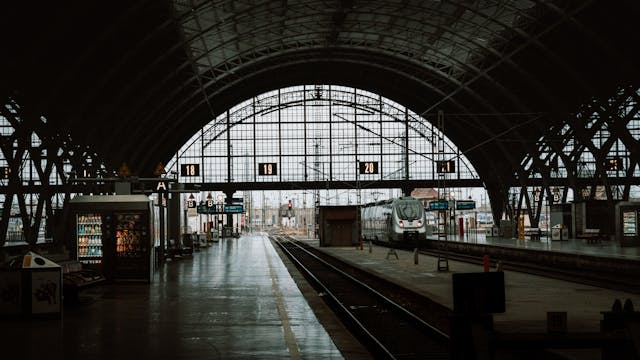
\includegraphics[width = 0.5\textwidth]{image/image.jpeg}
    \caption{Cool train station}
    \label{fig: image}
\end{figure*}



\end{ZhChapter}